\documentclass{standalone}
\usepackage{tikz}
\usetikzlibrary{patterns, positioning}


\begin{document}
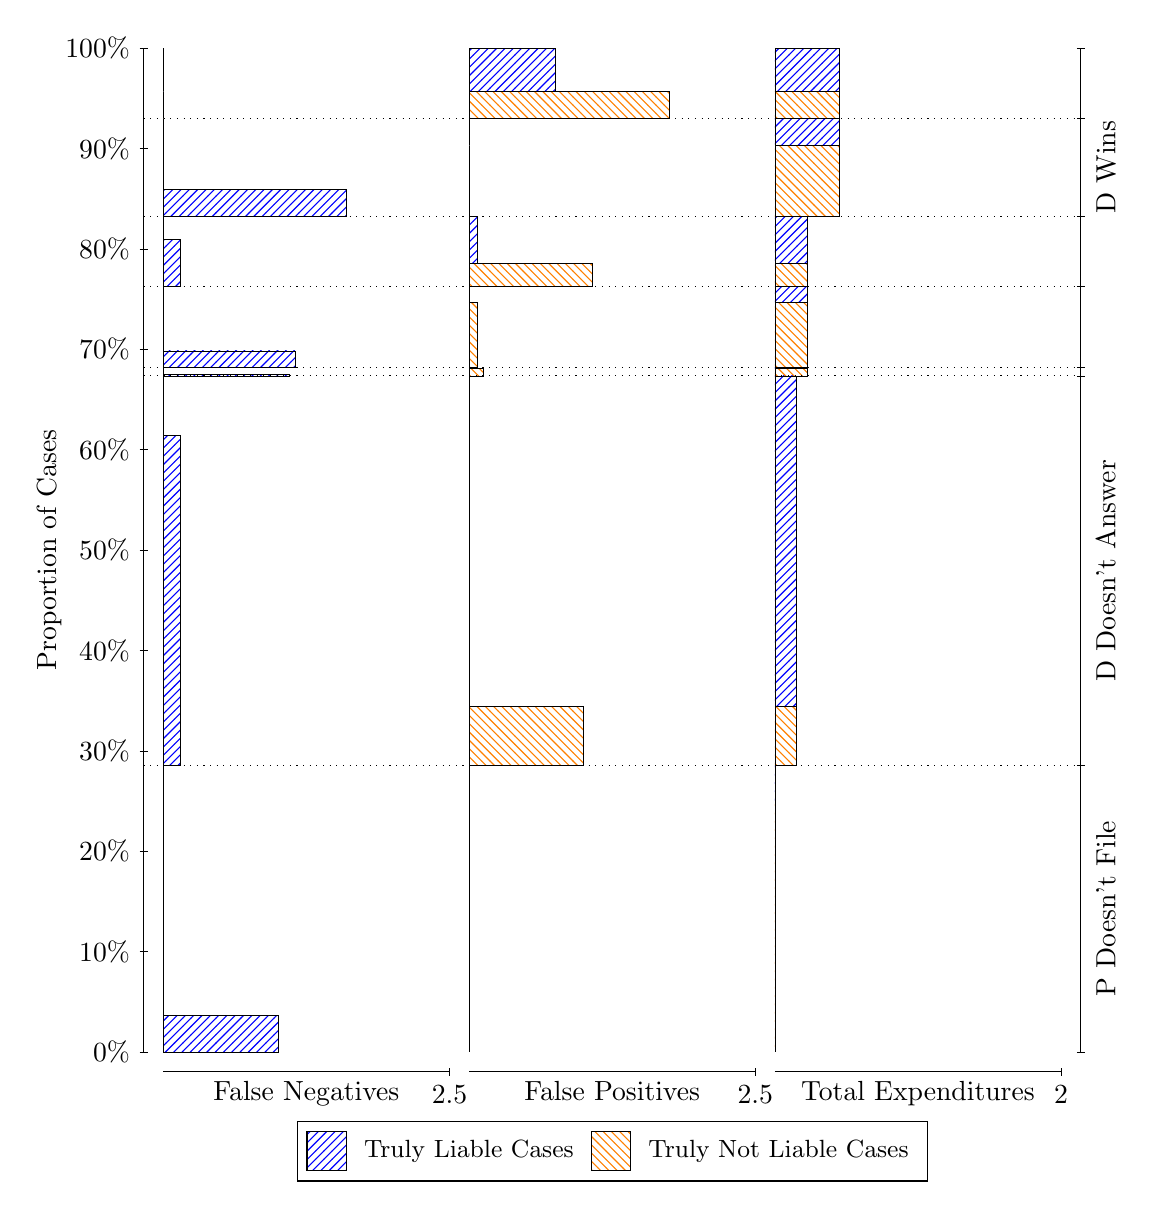
\begin{tikzpicture}
\draw[black, very thin] (1.5,1.75) -- (1.5,14.5);
\node[rotate=90, text=black, anchor=center] at (0.3, 8.125) {Proportion of Cases};
\draw[black, very thin] (1.45,1.75) -- (1.55,1.75);
\node[text=black, anchor=east] at (1.45, 1.75) {0\%};
\draw[black, very thin] (1.45,3.025) -- (1.55,3.025);
\node[text=black, anchor=east] at (1.45, 3.025) {10\%};
\draw[black, very thin] (1.45,4.3) -- (1.55,4.3);
\node[text=black, anchor=east] at (1.45, 4.3) {20\%};
\draw[black, very thin] (1.45,5.575) -- (1.55,5.575);
\node[text=black, anchor=east] at (1.45, 5.575) {30\%};
\draw[black, very thin] (1.45,6.85) -- (1.55,6.85);
\node[text=black, anchor=east] at (1.45, 6.85) {40\%};
\draw[black, very thin] (1.45,8.125) -- (1.55,8.125);
\node[text=black, anchor=east] at (1.45, 8.125) {50\%};
\draw[black, very thin] (1.45,9.4) -- (1.55,9.4);
\node[text=black, anchor=east] at (1.45, 9.4) {60\%};
\draw[black, very thin] (1.45,10.675) -- (1.55,10.675);
\node[text=black, anchor=east] at (1.45, 10.675) {70\%};
\draw[black, very thin] (1.45,11.95) -- (1.55,11.95);
\node[text=black, anchor=east] at (1.45, 11.95) {80\%};
\draw[black, very thin] (1.45,13.225) -- (1.55,13.225);
\node[text=black, anchor=east] at (1.45, 13.225) {90\%};
\draw[black, very thin] (1.45,14.5) -- (1.55,14.5);
\node[text=black, anchor=east] at (1.45, 14.5) {100\%};

\draw[black, very thin] (13.4,1.75) -- (13.4,14.5);
\draw[black, very thin] (13.35,1.75) -- (13.45,1.75);
\node[anchor=west] at (13.35, 1.75) {};
\draw[black, very thin] (13.35,5.3859) -- (13.45,5.3859);
\node[anchor=west] at (13.35, 5.3859) {};
\draw[black, very thin] (13.35,10.336) -- (13.45,10.336);
\node[anchor=west] at (13.35, 10.336) {};
\draw[black, very thin] (13.35,10.448) -- (13.45,10.448);
\node[anchor=west] at (13.35, 10.448) {};
\draw[black, very thin] (13.35,11.47) -- (13.45,11.47);
\node[anchor=west] at (13.35, 11.47) {};
\draw[black, very thin] (13.35,12.365) -- (13.45,12.365);
\node[anchor=west] at (13.35, 12.365) {};
\draw[black, very thin] (13.35,13.606) -- (13.45,13.606);
\node[anchor=west] at (13.35, 13.606) {};
\draw[black, very thin] (13.35,14.5) -- (13.45,14.5);
\node[anchor=west] at (13.35, 14.5) {};

\draw[black, very thin, pattern color=blue, pattern=north east lines] (1.75,1.75) rectangle (3.2033,2.2119);
\draw[black, very thin, pattern color=orange, pattern=north west lines] (1.75,2.2119) rectangle (1.75,5.3859);
\draw[black, very thin, pattern color=blue, pattern=north east lines] (1.75,5.3859) rectangle (1.968,9.5843);
\draw[black, very thin, pattern color=orange, pattern=north west lines] (1.75,9.5843) rectangle (1.75,10.336);
\draw[black, very thin, pattern color=blue, pattern=north east lines] (1.75,10.336) rectangle (3.3487,10.352);
\draw[black, very thin, pattern color=orange, pattern=north west lines] (1.75,10.352) rectangle (1.75,10.448);
\draw[black, very thin, pattern color=blue, pattern=north east lines] (1.75,10.448) rectangle (3.4213,10.653);
\draw[black, very thin, pattern color=orange, pattern=north west lines] (1.75,10.653) rectangle (1.75,11.47);
\draw[black, very thin, pattern color=blue, pattern=north east lines] (1.75,11.47) rectangle (1.968,12.07);
\draw[black, very thin, pattern color=orange, pattern=north west lines] (1.75,12.07) rectangle (1.75,12.365);
\draw[black, very thin, pattern color=blue, pattern=north east lines] (1.75,12.365) rectangle (4.0753,12.706);
\draw[black, very thin, pattern color=orange, pattern=north west lines] (1.75,12.706) rectangle (1.75,13.606);
\draw[black, very thin, pattern color=orange, pattern=north west lines] (1.75,13.606) rectangle (1.75,13.947);
\draw[black, very thin, pattern color=blue, pattern=north east lines] (1.75,13.947) rectangle (1.75,14.5);
\draw[black, very thin, pattern color=orange, pattern=north west lines] (5.6333,1.75) rectangle (5.6333,4.924);
\draw[black, very thin, pattern color=blue, pattern=north east lines] (5.6333,4.924) rectangle (5.6333,5.3859);
\draw[black, very thin, pattern color=orange, pattern=north west lines] (5.6333,5.3859) rectangle (7.0867,6.1372);
\draw[black, very thin, pattern color=blue, pattern=north east lines] (5.6333,6.1372) rectangle (5.6333,10.336);
\draw[black, very thin, pattern color=orange, pattern=north west lines] (5.6333,10.336) rectangle (5.815,10.432);
\draw[black, very thin, pattern color=blue, pattern=north east lines] (5.6333,10.432) rectangle (5.6333,10.448);
\draw[black, very thin, pattern color=orange, pattern=north west lines] (5.6333,10.448) rectangle (5.7423,11.265);
\draw[black, very thin, pattern color=blue, pattern=north east lines] (5.6333,11.265) rectangle (5.6333,11.47);
\draw[black, very thin, pattern color=orange, pattern=north west lines] (5.6333,11.47) rectangle (7.1957,11.764);
\draw[black, very thin, pattern color=blue, pattern=north east lines] (5.6333,11.764) rectangle (5.7423,12.365);
\draw[black, very thin, pattern color=orange, pattern=north west lines] (5.6333,12.365) rectangle (5.6333,13.265);
\draw[black, very thin, pattern color=blue, pattern=north east lines] (5.6333,13.265) rectangle (5.6333,13.606);
\draw[black, very thin, pattern color=orange, pattern=north west lines] (5.6333,13.606) rectangle (8.1767,13.947);
\draw[black, very thin, pattern color=blue, pattern=north east lines] (5.6333,13.947) rectangle (6.7233,14.5);
\draw[black, very thin, pattern color=orange, pattern=north west lines] (9.5167,1.75) rectangle (9.5167,4.924);
\draw[black, very thin, pattern color=blue, pattern=north east lines] (9.5167,4.924) rectangle (9.5167,5.3859);
\draw[black, very thin, pattern color=orange, pattern=north west lines] (9.5167,5.3859) rectangle (9.7892,6.1372);
\draw[black, very thin, pattern color=blue, pattern=north east lines] (9.5167,6.1372) rectangle (9.7892,10.336);
\draw[black, very thin, pattern color=orange, pattern=north west lines] (9.5167,10.336) rectangle (9.9254,10.432);
\draw[black, very thin, pattern color=blue, pattern=north east lines] (9.5167,10.432) rectangle (9.9254,10.448);
\draw[black, very thin, pattern color=orange, pattern=north west lines] (9.5167,10.448) rectangle (9.9254,11.265);
\draw[black, very thin, pattern color=blue, pattern=north east lines] (9.5167,11.265) rectangle (9.9254,11.47);
\draw[black, very thin, pattern color=orange, pattern=north west lines] (9.5167,11.47) rectangle (9.9254,11.764);
\draw[black, very thin, pattern color=blue, pattern=north east lines] (9.5167,11.764) rectangle (9.9254,12.365);
\draw[black, very thin, pattern color=orange, pattern=north west lines] (9.5167,12.365) rectangle (10.334,13.265);
\draw[black, very thin, pattern color=blue, pattern=north east lines] (9.5167,13.265) rectangle (10.334,13.606);
\draw[black, very thin, pattern color=orange, pattern=north west lines] (9.5167,13.606) rectangle (10.334,13.947);
\draw[black, very thin, pattern color=blue, pattern=north east lines] (9.5167,13.947) rectangle (10.334,14.5);
\draw[black, dotted] (1.5,5.3859) -- (13.4,5.3859);
\draw[black, dotted] (1.5,10.336) -- (13.4,10.336);
\draw[black, dotted] (1.5,10.448) -- (13.4,10.448);
\draw[black, dotted] (1.5,11.47) -- (13.4,11.47);
\draw[black, dotted] (1.5,12.365) -- (13.4,12.365);
\draw[black, dotted] (1.5,13.606) -- (13.4,13.606);
\draw[black, very thin] (1.75,1.5) -- (5.3833,1.5);
\node[text=black, anchor=north] at (3.5667, 1.5) {False Negatives};
\draw[black, very thin] (5.3833,1.45) -- (5.3833,1.55);
\node[text=black, anchor=north] at (5.3833, 1.45) {2.5};

\draw[black, very thin] (5.6333,1.5) -- (9.2667,1.5);
\node[text=black, anchor=north] at (7.45, 1.5) {False Positives};
\draw[black, very thin] (9.2667,1.45) -- (9.2667,1.55);
\node[text=black, anchor=north] at (9.2667, 1.45) {2.5};

\draw[black, very thin] (9.5167,1.5) -- (13.15,1.5);
\node[text=black, anchor=north] at (11.333, 1.5) {Total Expenditures};
\draw[black, very thin] (13.15,1.45) -- (13.15,1.55);
\node[text=black, anchor=north] at (13.15, 1.45) {2};

\node[text=black, centered, rotate=90] at (13.72, 3.568) {P Doesn't File};
\node[text=black, centered, rotate=90] at (13.72, 7.8608) {D Doesn't Answer};



\node[text=black, centered, rotate=90] at (13.72, 12.985) {D Wins};


\draw (7.449999999999999,1.5) node[draw=none] (baseCoordinate) {};
\begin{scope}[align=center]
        \matrix[scale=0.5, draw=black, below=0.5cm of baseCoordinate, nodes={draw}, column sep=0.1cm]{
            \node[rectangle, draw, minimum width=0.5cm, minimum height=0.5cm, pattern color=blue, pattern=north east lines] {}; &
            \node[draw=none, font=\small, text=black] (B) {Truly Liable Cases}; &
            \node[rectangle, draw, minimum width=0.5cm, minimum height=0.5cm, pattern color=orange, pattern=north west lines] {}; &
            \node[draw=none, font=\small, text=black] (B) {Truly Not Liable Cases}; \\
            };
\end{scope}

\end{tikzpicture}
\end{document}